% !TeX program = pdfLaTeX
\documentclass[12pt]{article}
\usepackage{amsmath}
\usepackage{amsthm}
\usepackage{amssymb}
\usepackage{bbm}
\usepackage{graphicx,psfrag,epsf}
\usepackage{enumerate}
%\usepackage[numbers]{natbib}
\usepackage[nomarkers]{endfloat}
\usepackage{natbib}
\setcitestyle{numbers} 
\makeatletter % Reference list option change
\renewcommand\@biblabel[1]{#1. } % from [1] to 1
\makeatother %

\usepackage{booktabs}
\usepackage{longtable}
\usepackage{array}
\usepackage{adjustbox}
\usepackage{multirow}
\usepackage{subfig}
\usepackage[table,xcdraw]{xcolor}
\usepackage{wrapfig}
\usepackage{float}
%\usepackage{colortbl}
\usepackage[colorlinks]{hyperref}
\hypersetup{
  colorlinks=true,
  citecolor=black,
  linkcolor=black,
  urlcolor=blue}
  
\usepackage{pdflscape}
\usepackage{tabu}
\usepackage{threeparttable}
\usepackage{url} % not crucial - just used below for the URL

\usepackage{etoolbox}% http://ctan.org/pkg/etoolbox
\makeatletter
\patchcmd{\subsection}{\bfseries}{\relax}{}{}% Non-bold \subsection
\patchcmd{\subsubsection}{\bfseries}{\relax}{}{}% Non-bold \subsection
\makeatother


%\pdfminorversion=4
% NOTE: To produce blinded version, replace "0" with "1" below.
\newcommand{\blind}{0}

% DON'T change margins - should be 1 inch all around.
\addtolength{\oddsidemargin}{-.5in}%
\addtolength{\evensidemargin}{-.5in}%
\addtolength{\textwidth}{1in}%
\addtolength{\textheight}{1.3in}%
\addtolength{\topmargin}{-.8in}%

\newenvironment{definition}[1]% environment name 
{% begin code 
  \par\vspace{.75\baselineskip}\noindent 
  \textbf{Definition (#1)}\begin{itshape}% 
  \par\vspace{.5\baselineskip}\noindent\ignorespaces 
}% 
{% end code 
  \end{itshape}\ignorespacesafterend 
}

\providecommand{\tightlist}{%
  \setlength{\itemsep}{0pt}\setlength{\parskip}{0pt}}

\begin{document}

\def\spacingset#1{\renewcommand{\baselinestretch}%
{#1}\small\normalsize} \spacingset{1}



%%%%%%%%%%%%%%%%%%%%%%%%%%%%%%%%%%%%%%%%%%%%%%%%%%%%%%%%%%%%%%%%%%%%%%%%%%%%%%

\if0\blind
{
  \title{\bf Statistical Approaches to Automated Groove Engraved Area Identification
in 3D Bullet Land Scans}

  \author{
        Kiegan Rice \thanks{The authors gratefully acknowledge \ldots{}} \\
    Department of Statistics, Iowa State University\\
     and \\     Nathaniel Garton \\
    Department of Statistics, Iowa State University\\
     and \\     Ulrike Genschel \\
    Department of Statistics and CSAFE, Iowa State University\\
     and \\     Heike Hofmann \\
    Department of Statistics and CSAFE, Iowa State University\\
      }
  \maketitle
} \fi

\if1\blind
{
  \bigskip
  \bigskip
  \bigskip
  \begin{center}
    {\LARGE\bf Statistical Approaches to Automated Groove Engraved Area Identification
in 3D Bullet Land Scans}
  \end{center}
  \medskip
} \fi

\bigskip
\begin{abstract}
Abstract will be written via the Gelman method once the introduction is
OK'd.
\end{abstract}

\noindent%
{\it Keywords:} 3 to 6 keywords, that do not appear in the title
\vfill

\newpage
\spacingset{1.45} % DON'T change the spacing!

\newcommand{\hh}[1]{{\color{orange}{#1}}}
\newcommand{\kr}[1]{{\color{teal}{#1}}}
\newcommand{\ug}[1]{{\color{purple}{#1}}}
\newcommand{\nate}[1]{{\color{olive}{#1}}}





TO DO:

\begin{itemize}
\tightlist
\item
  \kr{Abstract}
\end{itemize}

\section{Background}

Forensic pattern analysis aims to address the same-source problem:
whether two impressions were generated by the same object. One of the
most significant aspects of the same-source problem in firearms analysis
is the determination of whether two bullets were fired through the same
gun barrel. The evidence used in visual pattern comparison of bullets
are striation marks, which are engraved on the bullet by micro
imperfections in the barrel.

For barrels with traditional (i.e., not polygonal) rifling, striation
marks found on land engraved areas (LEAs) are the primary evidence used.
LEAs bear marks engraved by alternating sections of the barrel, and are
considered to be areas which will bear unique patterns of striation
marks which are reproduced on any bullet fired through the same barrel
\cite{AFTE}. \autoref{barrel-bullet} depicts lands inside a barrel, as
well as land engraved areas on a fired bullet.

The recent application of high resolution 3D scanning technology to
bullet LEAs coupled with concerns about the objectivity of visual
pattern comparison have motivated the development of several
image-analysis algorithms which aim to complete automated, quantitative
analyses of bullet evidence
\citep[see][]{DeKinder1, DeKinder2, Bachrach1, Ma1, Chu1, Chu2, Hare1}.
The data used in such algorithms are high resolution 3D scans of LEAs,
such as that pictured in \autoref{processing-process} (top).

Bullets can be algorithmically compared to one another by completing
individual LEA-to-LEA image comparisons of each LEA scan from one bullet
to each LEA scan from a second bullet. Each LEA-to-LEA pairing compares
the patterns of striation marks engraved on the LEA, which can be
extracted from a 3D scan as a 2D signature which details a pattern of
peaks and valleys representing striation marks.

Signatures are extracted by obtaining a horizontal slice of the 3D scan,
called a profile, followed by removing the overall bullet curvature
which dominates the data structure of each profile.
\autoref{processing-process} depicts the process of translating a 3D LEA
scan to a 2D LEA signature.

Currently accepted best practice for collecting 3D LEA scans involves
capturing portions of the neighboring groove engraved areas (GEAs),
introducing a secondary data structure on the edges of the LEA scan
which is not attributed to the pattern of interest: striation marks left
on the LEA.

In order to accurately represent the striation pattern as a 2D LEA
signature, the extraneous data structure introduced by GEA data must be
identified and removed. The identification of GEA data, while quite
straightforward for the human visual system, is a difficult process to
automate using computer vision techniques. A prior GEA identification
method was detailed as one step of the LEA matching algorithm proposed
in \citet{Hare1}. The method, ``rollapply'', uses data smoothing to
reduce noise measured in data and subsequently searches for the local
minima closest to the edges of each LEA. It often fails to adequately
identify large scale structural changes in favor of smaller structural
anomalies.

We describe here two methods for automated identification and removal of
GEA data. First, we use an adapted version of a robust statistical
modeling technique to remove bullet curvature. Then, we describe two
methods to separate GEA data from LEA data using statistical techniques.
We then assess performance of the two approaches on three separate test
sets of bullets by comparing performance of the \citet{Hare1} LEA
matching algorithm when each proposed method is applied within the
automated analysis pipeline.

\begin{figure}

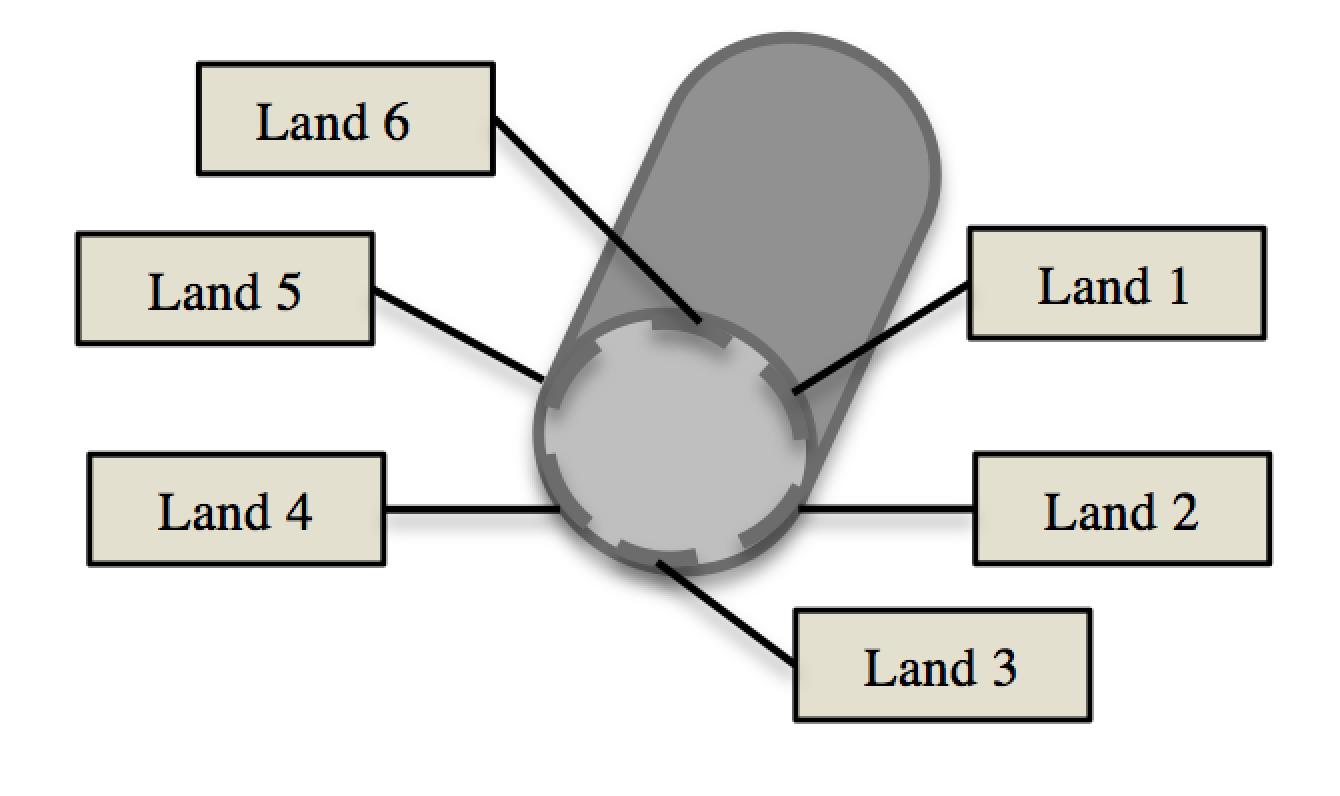
\includegraphics[width=0.5\textwidth]{../images/scanning-stage0}
\hspace{3cm}
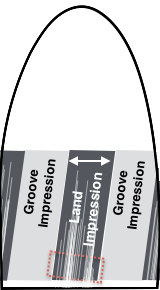
\includegraphics[width=0.2\textwidth]{../images/bullet-sketch}
\caption{(Left) A sketch depicting lands inside a traditionally rifled barrel with six lands. (Right) A sketch of a land engraved area and striation marks engraved on the bullet. Groove engraved areas are found between land engraved areas. The red area denotes the area of a bullet which would be captured as part of a LEA scan.}
\label{barrel-bullet}
\end{figure}

\begin{figure}
\centering
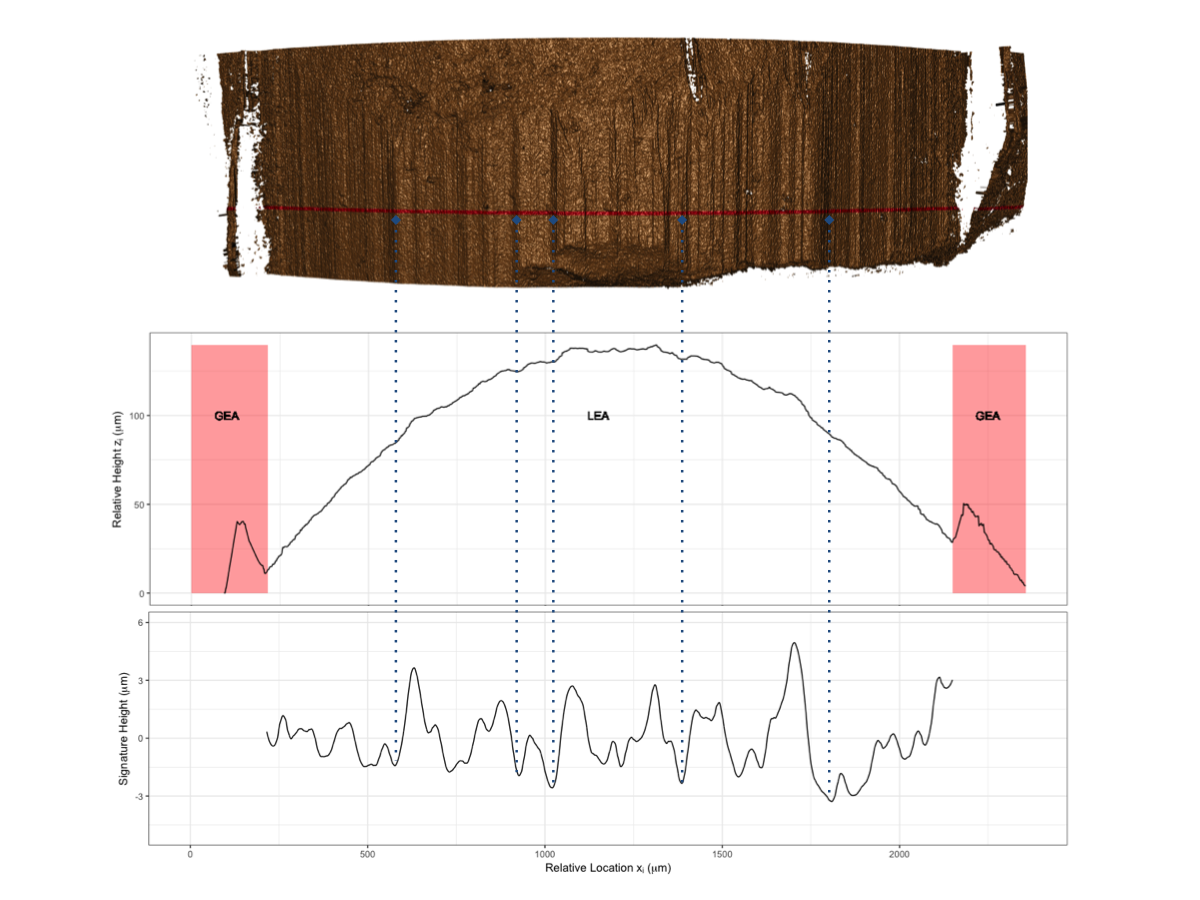
\includegraphics[width=\textwidth]{../images/process_vertical_png}
\caption{The process of extracting a 2D signature from a high-resolution 3D scan of a land engraved area (LEA) on a bullet. (Top) Computer rendering of a high-resolution 3D bullet LEA scan. Red line denotes horizontal crosscut which is extracted from the scan. (Middle) 2D extracted profile. Red boxes denote data which are part of the GEAs to the left and right sides of the LEA data. (Bottom) 2D extracted LEA signature with bullet curvature removed. Signatures are a representation of the striation pattern on each LEA. Vertical lines depict alignment of valleys with prominent striation marks.}  
\label{processing-process}
\end{figure}

\section{Data Source}

We use high resolution 3D scans of bullet LEAs. Scans were captured at
Iowa State University's High Resolution Microscopy Facility on a
Sensofar confocal light microscope at 20x magnification resulting in a
resolution of 0.645 microns per pixel. Scans are stored as x3p files,
conforming to the ISO5436-2 standard \citep{ISO5436}. x3p is the
industry standard format for capture and storage of 3D microscopic
topography of bullets. Objects are stored digitally as a 2-dimensional
matrix with \((x,y)\) locations corresponding to locations on the
physical object; a relative height value \(z\) is measured and recorded
for each \((x,y)\) location.

All six LEAs from each bullet were captured for bullets from three
separate test sets. Each test set contains a combination of ``known''
bullets, identified as originating from a particular gun barrel, and
``unknown'' bullets. In a closed test set, each unknown bullet
originates from one of the known barrels. In an open test set, unknown
bullets can originate from either a known barrel or a barrel outside of
the set entirely.

Hamby set 44 is a closed test set consisting of 35 bullets fired from 10
consecutively rifled Ruger P85 barrels. There are two known bullets for
each of the ten barrels, as well as 15 additional questioned bullets.
Every LEA was scanned for each of the 35 fired bullets in the set,
producing data for 210 individual land engraved areas. Two lands
\kr{-- Barrel 9, Bullet 2, Land 3 and Unknowns, Bullet L, Land 5 -- - remove?}
were removed from consideration due to ``tank rash''. Tank rash results
from a bullet striking the bottom of a water recovery tank after exiting
the barrel, thereby creating marks on the land that are not due to the
contact with the barrel.

The Phoenix PD set is a closed test set consisting of 33 bullets fired
from 8 barrels \kr{more information on the type of barrels?}. There are
three known bullets for each of the eight barrels, as well as 9
additional questioned bullets. Every LEA was scanned for each of the 33
fired bullets, producing a total of 198 individual land engraved areas.

The Houston-test set is an open test set consisting of 69 bullets fired
from more than 10 barrels \kr{more information on the type of barrels?}.
There are at least three known bullets for each of the ten barrels, with
a total of 33 known bullets. There are 24 questioned bullets that were
fired from a combination of the 10 known barrels and additional,
out-of-set barrels. Every LEA was scanned for each of the 69 fired
bullets, producing a total of 414 individual land engraved areas.

A vertical crosscut location was extracted from each scan by identifying
an optimal crosscut using \texttt{x3p\_crosscut\_optimize} in the
\texttt{bulletxtrctr} package in \texttt{R} \cite{bulletxtrctr}. We
calculated a profile by averaging across ten consecutive crosscuts which
fall directly to either side of the optimal crosscut identified. The
following GEA data identification methods are applied to these averaged
profiles, for a total of 820 profiles across the three test sets. In the
following, we utilize relative horizontal locations on the profile,
\(x_i\), and their relationship with relative height values on the
profile, \(z_i\), for data points \(i = 1, ..., n\) on each individual
profile.

\section{Methodology}

We propose two methods for separating GEA data from LEA data. One
method, logistic LASSO, uses supervised two-class classification
techniques to classify each data point as being part of the LEA or GEA.
The second approach is Bayesian changepoint analysis, an unsupervised
method that seeks to identify data points where the distribution of the
residuals changes. Both methods require first removing the global
structure of the LEA scan, a non-trivial statistical procedure we will
describe before further developing each method.

\subsection{Global Structure Removal}

The first stage of both GEA removal process requires removing the bullet
curvature from each profile. GEAs on the edge of each LEA represent a
change in the primary data structure typically characterized by a sharp
increase in measured height values, as demonstrated in
\autoref{processing-process} (middle). Removal of the primary curvature
should leave the secondary structure intact -- namely, the sharp
increase in height values. The increase in values can then be used to
separate LEA data from GEA data.

Bullets are subjected to significant pressure in the process of being
fired through a gun barrel. Thus, we cannot assume completely circular
curvature on bullet LEAs. Further, we cannot model bullet curvature as a
directly circular structure. We use more flexible non-parametric locally
weighted regression (LOESS), which can model large-scale structure of
the height values \(z_i\). LOESS is flexible enough to model structural
defects within the bullet curvature. However, the flexibility also
leaves LOESS susceptible to modeling the secondary structure of the GEA.

Traditional LOESS predicts height values \(\widehat{z}_i\) as a function
of location \(x_i\) by estimating values \(\beta_0, \beta_1\) which
minimize:

\[ \arg\min_{\beta} \sum_{k=1}^n w_k(x_i) (z_k - (\beta_0 + \beta_1x_k))^2,\]

where \(w_k(x_i)\) is a weight assigned to each data point \(x_k\) based
on its proximity to \(x_i\). Weights \(w_k\) decrease as distance to
\(x_i\) increases, so that data points closest to \(x_i\) influence the
prediction \(\widehat{z}_i\) most. Weights \(w_k(x_i)\) are defined
using a prespecified decreasing function, traditionally a tricube
weight.

An alternative approach which mitigates the impact of GEA data is robust
LOESS (see \cite{Cleveland1}), a process which iteratively updates
weights \(w_k(x_i)\) by multiplying by a robustness weight, \(\delta_k\)
based on the magnitude of each residual \(e_k = z_k - \widehat{z}_k\).
Larger values of \(e_k\) result in a lower weight for that data point,
\(z_k\). The process is as follows:

\begin{enumerate}

\item Fit a LOESS model to a LEA profile, predicting height $z_i$ using relative location $x_i$. Assign robustness weights $\delta_k$ of 1 to each data point $(x_k, y_k)$.  
\item Obtain predicted height values $\widehat{z}_k$, and corresponding residual values $e_k = z_k - \widehat{z}_k$. 
\item Calculate updated robustness weights using residual values $e_k$: 

$$\delta_k \times w_k(x_i) =\left(1 - \left(\frac{e_k}{6*MAD}\right)^2\right)^2 \times w_k(x_i) \quad \quad \mbox{if}\quad \left|\frac{e_k}{6*MAD} \right| < 1,$$

where $MAD$ is the median absolute deviation of residuals $e_k$. This is known as the bisquare function.  
\item Repeat steps 1-3 with updated weights at each iteration for $m$ iterations, with 20 iterations as the default.  
\item After $m$ iterations of updating the weight vector $\delta_k w_k(x_i)$, fit a LOESS model and obtain residual values $e_i$ for each data point $(x_i, z_i)$.  

\end{enumerate}

Re-weighting data as in Step 3 reduces influence of data points with
large absolute residual values. When GEA data is present on a profile,
largest residual values will occur in areas where GEA data begins as it
presents a competing structure with overall LEA curvature.

\autoref{loess-vs-locfit} depicts the impact this iterative re-weighting
process has on curvature removal for an example LEA from Hamby set 44.
Predictions \(\widehat{z}_i\) are updated and more closely follow the
primary structure of bullet curvature.

However, this method fails to mitigate GEA data impact when GEA
structures are more pronounced. Thus, we make a small adaptation to the
procedure to function more effectively with these data structures, such
as the one in \autoref{houston-adapted-rlo-pdf}:

\begin{enumerate}

\item Fit a LOESS model to a LEA profile, predicting height $z_i$ using relative location $x_i$. Assign robustness weights $\delta_k$ of 1 to each data point $(x_k, y_k)$.  
\item Obtain predicted height values $\widehat{z}_k$, and corresponding residual values $e_k = z_k - \widehat{z}_k$. 
\item Calculate updated robustness weights using residual values $e_k$: 

$$\delta_k \times w_k(x_i) =\left(1 - \left(\frac{e_k}{6*MAD}\right)^2\right)^2 \times w_k(x_i) \quad \quad \mbox{if}\quad \left|\frac{e_k}{6*MAD} \right| < 1,$$

where $MAD$ is the median absolute deviation of residuals $e_k$. $\delta_k$ is known as the bisquare function.  
\item Assign updated weights as in Step 3 if $e_k > 0$. Else, leave weights as $w_k(x_i)$. 
\item Repeat steps 1-4 with updated weights at each iteration for $m$ iterations, with 20 iterations as the default.  
\item After $m$ iterations of updating the weight vector $w_k(x_i)$, fit a LOESS model and obtain residual values $e_i$ for each data point $(x_i, z_i)$.  

\end{enumerate}

This adapted robust LOESS, while a small procedural change, more adeptly
fits bullet curvature. \autoref{houston-adapted-rlo-pdf} demonstrates
the impact of the adaptation on predicted height values \(z_i\) and
residual value \(e_i\). \autoref{adapted-rlo-shift} depicts the
differing levels of impact our adjustment has on each bullet test set.
\kr{Once I have more barrel information, I could go into a little more detail here about differing barrel types/ammo types or something, but no more than a sentence to bring the point home.}

Once the adapted robust LOESS procedure has been applied to a LEA
profile, the resulting residuals \(e_i\) follow a reliable pattern:
small residuals closer to zero in locations associated with LEA data,
and sharply increasing, larger residuals in locations associated with
GEA data. The resulting residual structure lends itself to statistical
techniques to separate the two structures more effectively.

The subsequent GEA identification methods are based on residuals \(e_i\)
calculated from adapted robust LOESS fit to the global structure of the
profile. Both methods result in ``shoulder location predictions'',
predictions for the locations \((x_L, x_R)\) at which LEA data ends and
GEA data begins on the left and right side of the profile, respectively.

\begin{figure}
\centering
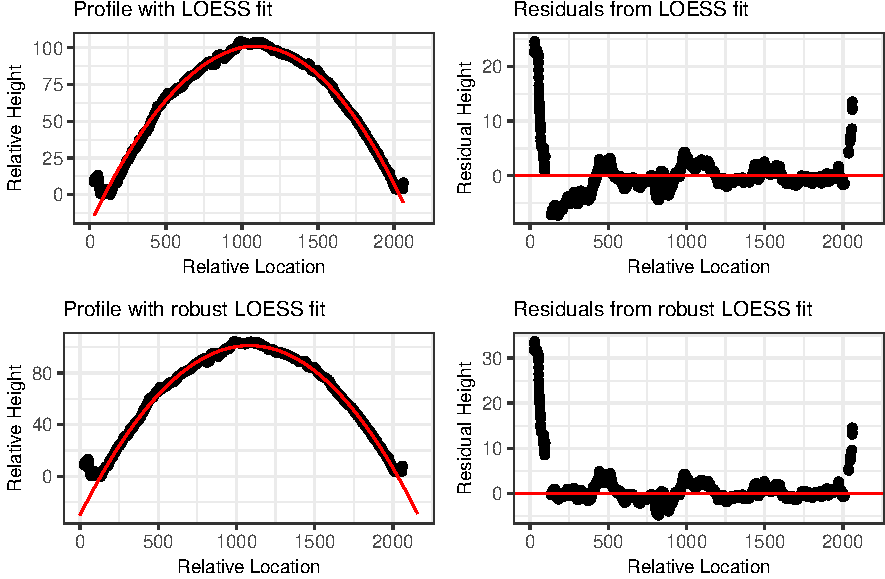
\includegraphics{writeup_files/figure-latex/loess-vs-locfit-1.pdf}
\caption{\label{loess-vs-locfit}An example of the difference between
traditional LOESS fit and robust LOESS fit to an LEA profile from Hamby
set 44.}
\end{figure}

\begin{figure}
\centering
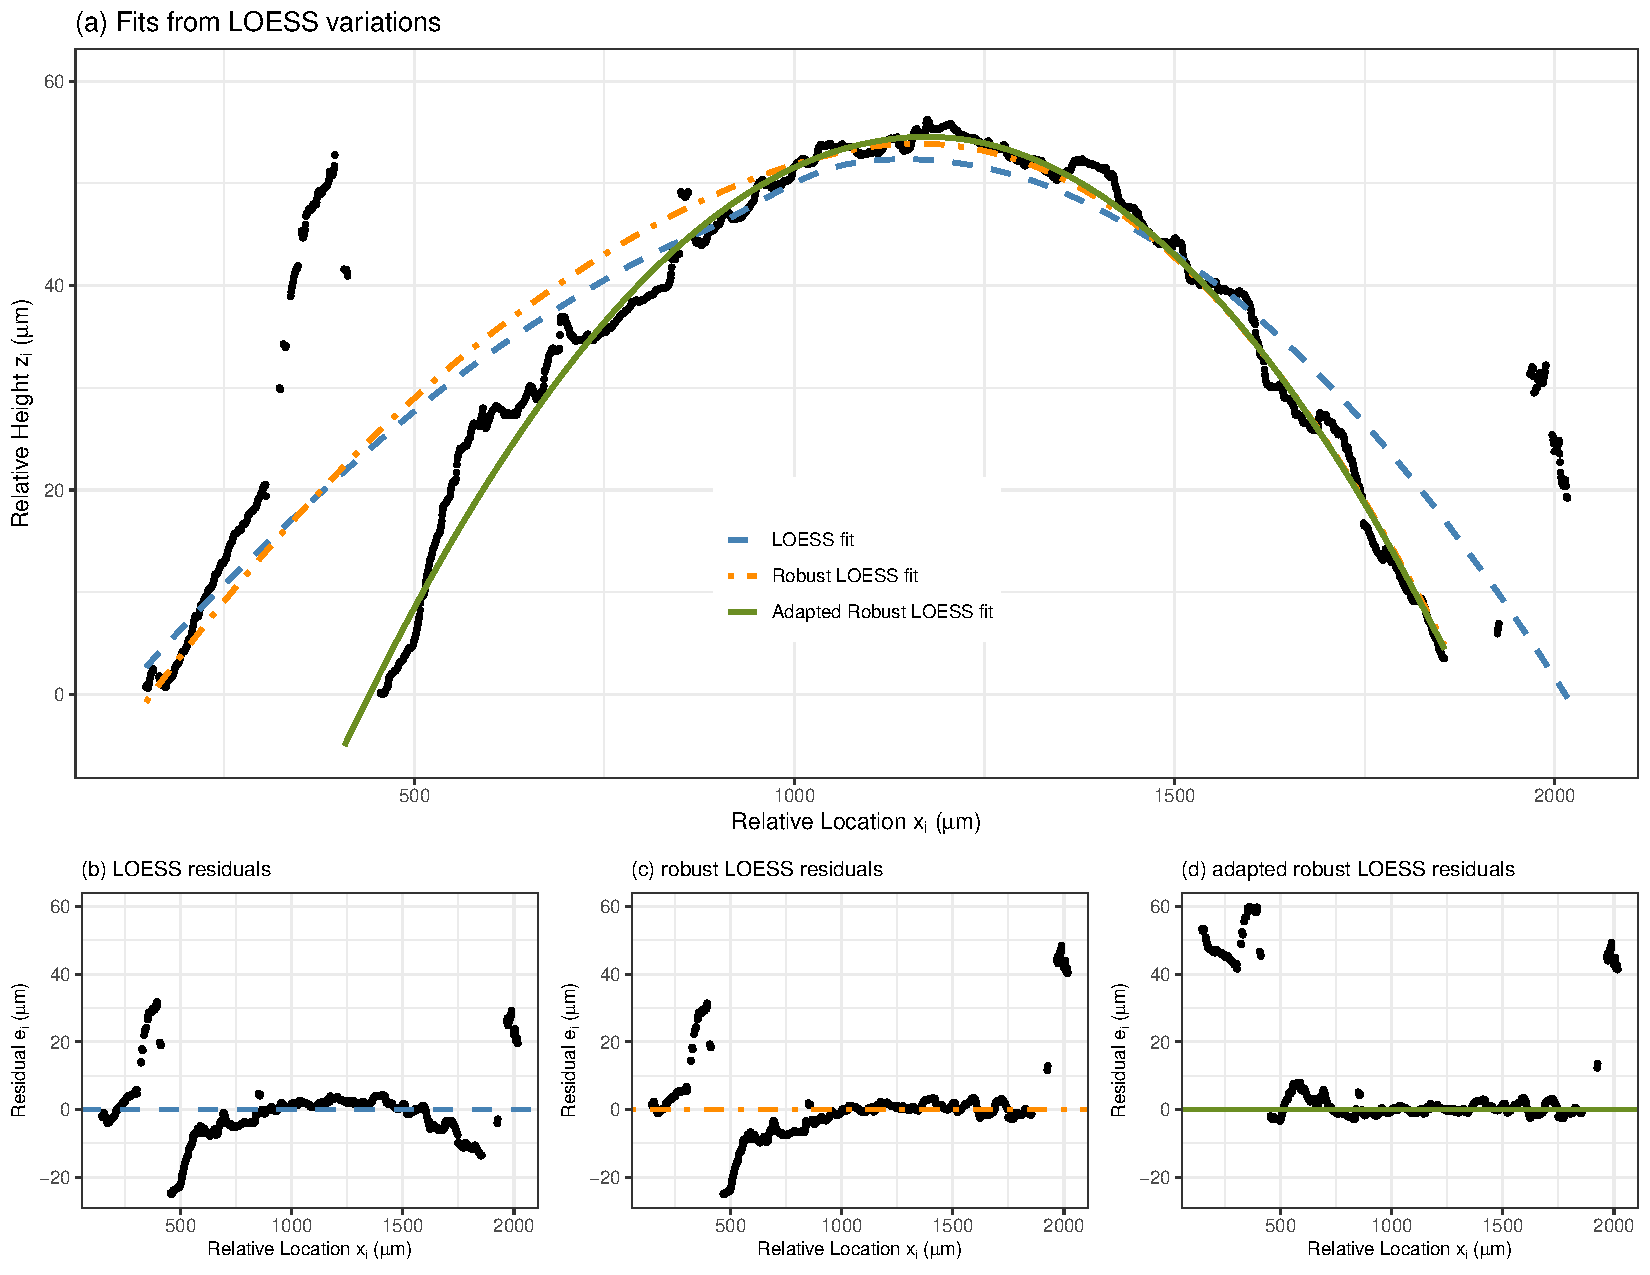
\includegraphics[width=\textwidth]{../images/loess_comparison_plot_all_wide}
\caption{An example of the difference between LOESS, robust LOESS, and adapted robust LOESS fits to an LEA profile from the Houston-test set. (a) depicts predicted curves for all three methods on one LEA. Adapted robust LOESS most closely fits the LEA structure and allows GEA data to remain a separate structure. (b), (c), and (d) depict residuals $e_i$ resulting from each respective prediction method. Adapted robust LOESS in (d) results in the most desirable residual pattern, with LEA data residuals remaining closer to zero, and GEA data residuals being positive and large.}
\label{houston-adapted-rlo-pdf}
\end{figure}

\begin{figure}
\centering
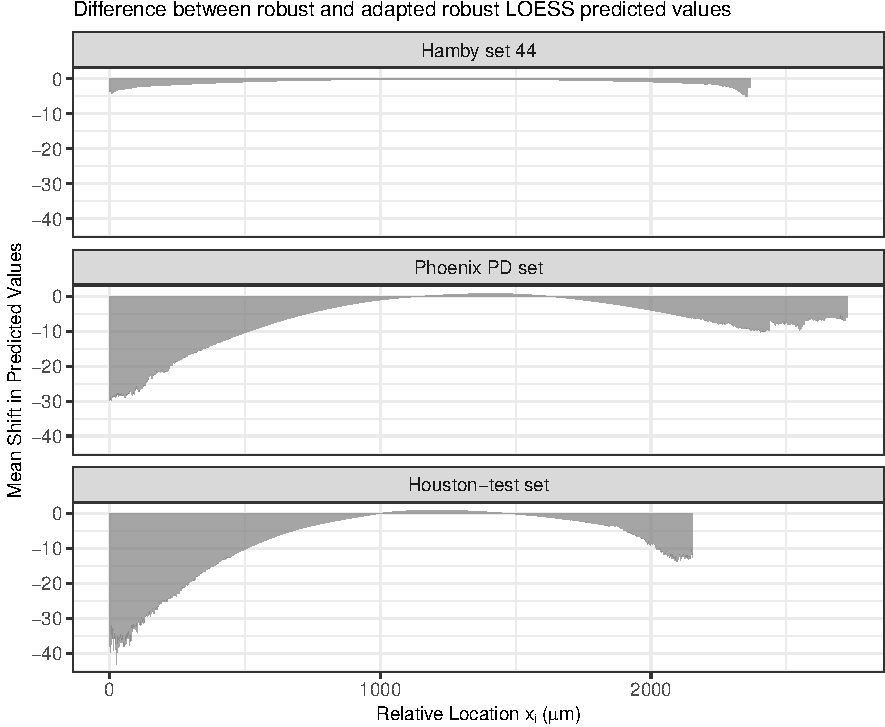
\includegraphics{writeup_files/figure-latex/adapted-rlo-shift-1.pdf}
\caption{\label{adapted-rlo-shift}Mean shift in predictions when
applying the adapted robust LOESS procedure in place of the traditional
robust LOESS procedure. For Hamby set 44 predictions are, on average,
very similar. The Phoenix PD and Houston-test sets have more significant
downwards shifts in predictions near the left and right boundaries.}
\end{figure}

\subsection{Logistic LASSO}

Shoulder location can be predicted by first classifying each residual
points as one of two classes (``LEA'' or ``GEA''), and subsequently
gathering the range of values classified as ``LEA'' points.

Classification into ``LEA'' or ``GEA'' is first approached by a process
of feature engineering based on adapted robust LOESS residuals. While
the residuals \(e_i\) should demonstrate differing patterns of
magnitude, residuals alone are not enough to classify data with high
accuracy.

\begin{figure}
\centering
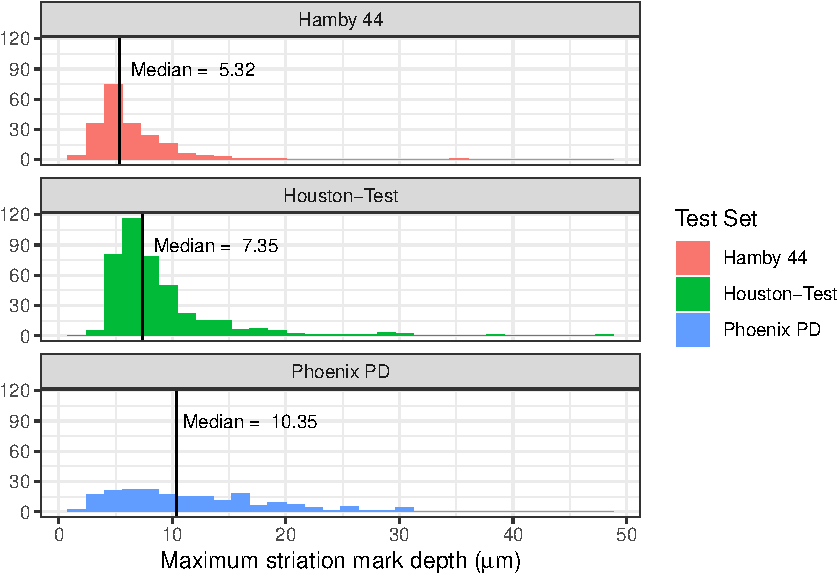
\includegraphics{writeup_files/figure-latex/striae-magnitudes-1.pdf}
\caption{\label{striae-magnitudes}Distribution of maximum striation
depth for each of the three bullet test sets. Maximum striation depths
are calculated as the largest observed absolute signature value in each
individual LEA signature. Black vertical lines represent the median
depth for each test set. Each test set has a different distribution,
which indicates standardization of residual heights is crucial for
generalizability of parameter estimates.}
\end{figure}

\autoref{striae-magnitudes} demonstrates that each test set has distinct
patterns of striation depth. Thus, standardization of features is
imperative for transferability of fitted model parameters. The LEA scan
context requires some non-traditional standardization practices.

For example, consider the distribution of residual values \(e_i\)
resulting from adapted robust LOESS. There is reason to believe that the
distribution will be quite skewed, which means a standard deviation will
not be a good proxy for the spread of the distribution. Thus, rather
than the standard deviation, we consider instead the standard deviation
of residual values from the middle 50\% of \(x_i\) values present in
each profile. This alternative acts as a proxy for the depth of striae
on each LEA, with higher standard deviations found for lands with deeper
striae. Standardizing residual values by this proxy puts all residuals
on a comparable scale.

For variables that deal with differences in the \(x\) direction, such as
depth from the center of a scan, values will be mapped to a \((0, 1)\)
range.

The full list of standardized features are as follows:

\begin{itemize}

\item[] \textbf{Standardized residuals $e_i$} \kr{(\texttt{rlo\_resid\_std})}: Robust LOESS residual value $e_i$, standardized by dividing by standard deviation of residual values from middle 50\% of $\mathbf{x_i}$ values.  

\item[] \textbf{Standardized residuals squared, $e_i^2$} \kr{(\texttt{(rlo\_resid\_std$\mathbf{)^2}$})}: Squared term of \texttt{rlo\_resid\_std}.   

\item[] \textbf{Side of scan} \kr{(\texttt{side})}: Whether data point is to left or right of median $x_i$ value.  

\item[] \textbf{Standardized depth from scan center} \kr{(\texttt{depth\_std})}: Distance of data point from median $x_i$ value, standardized by dividing by maximum $x_i$ value (a proxy for the range of $x$ values).  

\item[] \textbf{Side of scan, depth interaction} \kr{(\texttt{side:depth\_std})}: Interaction between \texttt{side} and \texttt{depth\_std} variables.  

\item[] \textbf{Left $x_i$ intercept} \kr{(\texttt{xint1\_std})}: Predicted location $x_i$ at which adapted robust LOESS crosses $y$ axis on left side of profile, standardized by dividing by maximum $x_i$ value (a proxy for the range of $x$ values).  

\item[] \textbf{Right $x_i$ intercept} \kr{(\texttt{xint2\_std})}: Predicted location $x_i$ at which adapted robust LOESS crosses $y$ axis on right side of profile, standardized by dividing by maximum $x_i$ value (a proxy for the range of $x$ values).  

\item[] \textbf{Range of local residuals $e_i$} \kr{(\texttt{range\_50\_std})}: Range of residual values $e_i$ within a 50-point window $(x_{i-25}, x_{i+25})$ around data point $x_i$, standardized by dividing by standard deviation of residual values from middle 50\% of $x_i$ values.  

\item[] \textbf{Number of local missing values} \kr{(\texttt{numNA\_50})}: Number of missing values within a 50-point window $(x_{i-25}, x_{i+25})$ around data point $x_i$.  

\item[] \textbf{Magnitude indicator for residual $e_i$} \kr{(\texttt{ind\_2mad})}: Indicator of whether \texttt{rlo\_resid} is greater than \texttt{2*MAD(rlo\_resid)}, where $MAD$ is the median absolute deviation of residual values $e_i$ for an entire profile.    

\item[] \textbf{Number of local positive $e_i$ values} \kr{(\texttt{numpos\_50})}: Number of positive residual values within a 50-point window $(x_{i-25}, x_{i+25})$ around data point $x_i$.  

\item[] \textbf{Outside edges indicator} \kr{(\texttt{ind\_edges})}: Indicator of whether data point is to the left of \texttt{xint1} or to the right of \texttt{xint2}. Values between \texttt{xint1} and \texttt{xint2} receive a value of 0, while values on the outside of the two values receive a value of 1.  

\end{itemize}

Examples of the distributions of some of these features can be seen in
\autoref{lasso-features}.

\begin{figure}
\centering
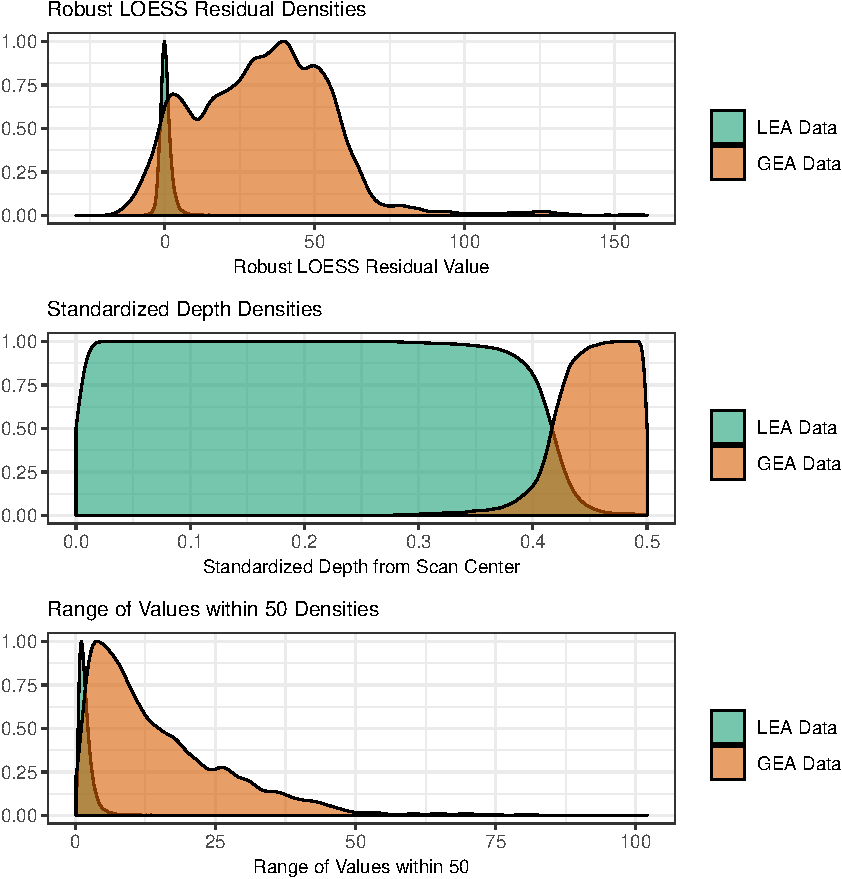
\includegraphics{writeup_files/figure-latex/lasso-features-1.pdf}
\caption{\label{lasso-features}Example distributions of features used in
two-class classification from Hamby set 44. While depth shows the most
clear separation between GEA and LEA data, it alone will not suffice to
classify data correctly.}
\end{figure}

A logistic LASSO model, a form of penalized regression, was fit using
the developed features. LASSO parameter values for \(p\) covariates were
calculated by identifying:\\
\[
\hat{\beta}_{\lambda} = \stackrel{\arg\min}{\beta \in \mathbb{R}^p} \left\{  (Y - X\beta)'(Y - X\beta) + \lambda \sum_{j=1}^{p}|\beta_j|\right\},
\] where \(X\) is a matrix with \(n\) rows, and a column for each data
feature described above. \(\beta\) is a vector of estimated parameter
values associated with each data feature, and \(Y\) is the vector of
length \(n\) of response class values, either a 1 for GEA class, or a 0
for LEA class. LASSO adds a penalty to the traditional ordinary least
squares minimization problem, and uses a tuning parameter \(\lambda\)
\citep{LASSO}. Predicted probabilities of membership in the GEA class
can be calculated as:

\[ \widehat{p_i} = \frac{\exp\{ X\hat{\beta_{\lambda}}\}}{1 + \exp \{X\hat{\beta_{\lambda}}\}}.\]

A cross-validated logistic LASSO model was fit using the
\texttt{cv.glmnet} function in the \texttt{glmnet} package in \texttt{R}
\cite{glmnet}. Parameter values from the model with \(\lambda_{1se}\)
were used. \(\lambda_{1se}\), a standard when using LASSO, is the tuning
parameter which results in the simplest model that still has
cross-validation error within one standard deviation of the best model.

The resulting model uses each of the data features listed above along
with pairwise interactions for each of them. The \(\hat{\beta}\) vector
was estimating using Hamby set 44 data. Parameter values were used to
calculate predicted values of GEA membership between 0 and 1; the closer
to 1, the higher probability of membership in the ``GEA'' class.

Two-class classification techniques traditionally employ a cutoff for
predicted probabilities and assign predicted class membership using that
cutoff; i.e., values above a certain cutoff are classified as part of
the ``GEA'' class, and values below the cutoff are classified as part of
the ``LEA'' class. An equal error rate is typically used for this
purpose. Equal error rate is defined as the cutoff at which sensitivity
(true positive rate) and specificity (true negative rate) are equal.
However, since LEA scans consist of a majority of LEA data by nature,
significant class imbalance in our response variable (``GEA'' vs.
``LEA'') dictates a change in procedure for assigning a cutoff for class
membership. Employing an equal error rate cutoff to predict class
membership would result in a higher number of false positives, here
predicting data which is part of the ``LEA'' class as ``GEA'' data. We
employ an equal \textit{number of errors} rate rather than an equal
error rate to ameliorate this imbalance.

The pipeline of this method for shoulder location identification is as
follows:

\begin{enumerate}
\item Use adapted robust LOESS procedure to remove bullet curvature and obtain residual values $e_i$.
\item Extract data features based on $x_i$ locations and residual height values $e_i$ from Step 1. 
\item Use fit parameter values from trained logistic LASSO model to calculate probabilities of membership in GEA class. 
\item Apply cutoff of $.34$: classify higher probabilities as GEA data points, and lower probabilities as LEA data points.
\item Identify the minimum $x_i$ value which is predicted as a member of the LEA class, $x_{L}$. Identify the maximum $x_i$ value which is predicted as a member of the LEA class, $x_{R}$. $(x_L, x_R)$ are the shoulder location predictions.  
\end{enumerate}

This method for shoulder location identification can be found in the
\texttt{R} package \texttt{bulletxtrctr} as the function
\texttt{get\_grooves\_lassofull}. \kr{Another method,}
\texttt{get\_grooves\_lassobasic}, \kr{is also available through}
\texttt{bulletxtrctr},
\kr{but is slightly less accurate and thus is not laid out here.}

\subsection{Bayesian Changepoint Analysis}

Our second approach is also based on the idea that residuals \(e_i\)
resulting from adapted robust LOESS predictions will follow a consistent
pattern: decreasing values in the left GEA, values with no discernable
slope change in the LEA, and increasing values in the right GEA. This
can be thought of as a line with negative slope for the left GEA, line
with zero slope for the LEA, and a line with positive slope for the
right GEA. The next model will therefore be defined in a piecewise
fashion. The points of global structural change are what we will call
changepoints. Changepoint locations can be treated as unknown parameters
and estimated in the same manner as any other parameter in a statistical
model.

Identifying such structural points was proposed more generally as
Bayesian changepoint detection in \citet{stephens1994}. In the context
of LEA residuals, there are additional complex patterns (i.e., striation
marks), but the overall linear structure remains on a larger scale. We
will consider the smaller scale striation patterns as dependence in the
data after accounting for the large scale structures we are estimating.

We first perform some additional data processing steps to streamline
computation. First, we scale the residuals \(e_i\) from the robust LOESS
procedure by dividing by the standard deviation of residuals \(e_i\) for
the entire profile. The purpose of this is purely to make certain priors
easier to specify. Secondly, we impute missing residual values \(e_i\)
to maintain equidistance between \(x_i\) locations.

We next develop a model which we will use to identify changepoints, and
describe estimation procedures. Additional details on data processing
can be found in the appendix.

\subsubsection{Bayesian Model Formulation}

For model formulation, we will define random variables associated with
residual values \(e_i\). Let \(\{Y(x_i): i = 1,2, ..., n\}\) denote the
set of random variables representing the residuals from the robust LOESS
procedure at the values \(x_i\). Also assume that
\(x_1 < x_2 < ... < x_n\). Let \(c_l\) be the value of the left
changepoint and \(c_r\) be the value of the right changepoint. Here, the
left changepoint is where the left GEA meets the LEA, and the right
changepoint is where the right GEA meets the LEA. Denote the median
centered \(x\) values as \(x'_i = x_i - \tilde{x}\) where \(\tilde{x}\)
is the median \(x\) value. Complex small scale patterns, such as the
striae, will be modeled through a covariance structure on the data that
will be allowed to differ between each GEA and between the GEAs and LEA.
We will construct the covariance matrices from the exponential
covariance function
\(K(x, x';\sigma, \ell) = \sigma^2 e^{-\frac{|x - x'|}{\ell}} = cov(Y(x), Y(x'))\).
The differences in covariance matrices for the GEAs and LEA will be
reflected in the parameters \(\sigma\) and \(\ell\). The data model that
we consider is then,

\begin{align}
(Y(x_1), Y(x_2), ..., Y(x_{k_1}))^{\top} &\sim N(\beta_{01}\mathbbm{1} + \beta_{11} x_{1:k_1}, \Sigma_1(\sigma_1, \ell_1)) \\
(Y(x_{k_1 + 1}), Y(x_{k_1 + 2}), ..., Y(x_{k_2}))^{\top} &\sim N(0, \Sigma_2(\sigma_2, \ell_2)) \\ 
(Y(x_{k_2 + 1}), Y(x_{k_2 + 2}), ..., Y(x_n))^{\top} &\sim N(\beta_{02}\mathbbm{1} + \beta_{12} x_{k_2 + 1:n}, \Sigma_3(\sigma_3, \ell_3)),
\end{align}

\noindent where \(x_{k_1} < c_l \leq x_{k_1 + 1}\) and
\(x_{k_2} < c_r \leq x_{k_2 + 1}\) Here, \(x_{1:k}\) denotes the column
vector \((x_1, x_2, ..., x_k)^\top\), and \(\mathbbm{1}\) denotes the
vector of ones. Independence is assumed between each of these three
distributions for two reasons. Firstly, it simplifies the computations
significantly. Secondly, the robust loess residual values are the sum of
the relevant global structure (GEA or LEA) and finer local structure
(e.g.~striae). The global structure component of any two residual values
should be independent conditioned on the known global structure at the
location of each residual. The local structure tends to be meaningful
only over small regions of the land, and so any dependence between the
GEAs and LEA due to local structure should be small enough to safely
ignore. The parameters that need to be estimated include the four mean
parameters in the GEAs, the six covariance parameters (two for each of
the three areas), and the two changepoint parameters, \(c_l\) and
\(c_r\).

The above model encapsulates the essence of the approach. However, there
are a few difficulties. The first difficulty is that there are not
always two GEAs in a particular land. There may be one GEA, or the land
may only consist of the LEA. Thus, the above model is conditional on
there being two GEAs in the data. We also define models for when there
is one GEA on the left, one GEA on the right, or no GEAs. The models are
defined in an essentially identical way. Conditional on there being only
one GEA, the left GEA model is defined as,

\begin{align}
(Y(x_1), Y(x_2), ..., Y(x_{k}))^{\top} &\sim N(\beta_{0}\mathbbm{1} + \beta_{1} x_{1:k}, \Sigma_1(\sigma_1, \ell_1)) \\
(Y(x_{k + 1}), Y(x_{k + 2}), ..., Y(x_{n}))^{\top} &\sim N(0, \Sigma_2(\sigma_2, \ell_2)),
\end{align}

\noindent and the right GEA model is defined as,

\begin{align}
(Y(x_{1}), Y(x_{2}), ..., Y(x_{k}))^{\top} &\sim N(0, \Sigma_1(\sigma_1, \ell_1)) \\ 
(Y(x_{k + 1}), Y(x_{k + 2}), ..., Y(x_n))^{\top} &\sim N(\beta_{0}\mathbbm{1} + \beta_{1} x_{k + 1:n} \Sigma_2(\sigma_2, \ell_2)).
\end{align}

\noindent Finally, conditional on there being no GEAs in the data, the
model is simply

\begin{align}
(Y(x_{1}), Y(x_{2}), ..., Y(x_{n}))^{\top} &\sim N(0, \Sigma(\sigma, \ell)).
\end{align}

Estimating the changepoint locations also involves selecting the most
appropriate model from these four. We use \(m_0\) to denote the model
with no GEA, \(m_{1l}\) and \(m_{1r}\) to denote the models with one
left or one right GEA, respectively, and we use \(m_2\) to denote the
model with two GEAs. In order to avoid confusion, we have slightly
abused notation and, for example, \(\Sigma_1(\sigma_1, \ell_1)\) as it
is estimated in the two changepoint model is \emph{not} the same as
\(\Sigma_1(\sigma_1, \ell_1)\) from either of the one changepoint
models, and \(\Sigma_1(\sigma_1, \ell_1)\) is also \emph{not} the same
between the two one changepoint models. As another example, \(\beta_0\)
is \emph{not} the same between each of the one changepoint models. So,
to be clear, duplication of notation in \emph{different} models is not
meant to imply that those parameters are shared between models.

Ultimately, models \(m_0\), \(m_{1l}\), \(m_{1r}\), and \(m_2\) are each
given a prior and individually fitted on every profile. From there, we
do model selection in the formal Bayesian way, selecting number and
location of changepoints by maximizing the estimated posterior
distribution.

In order to complete a Bayesian model specification, we need priors on
the parameters in each model as well as the model itself. We will assume
independence between each parameter a priori. For each length scale
\(\ell\), we will assume \(\ell \sim \text{Gamma}(3,5)\). For each
standard deviation, we will assume
\(\sigma \sim \text{Half-Normal}^{+}(0,1)\), where
\(\text{Half-Normal}^{+}(\cdot,\cdot)\) is notation for the normal
distribution restricted to the positive real numbers. For intercept
parameters, \(\beta_{01}, \beta_{02}, \beta_0 \sim N(0, 10)\). For the
slope parameters, the preceding trend deviates slightly. For any slope
that corresponds to the \emph{left} GEA, \(\beta_1\) or \(\beta_{01}\),
we will assume that the slope can not be positive. That is,
\(\beta_1, \beta_{01} \sim \text{Half-Normal}^{-}(0,10)\), where
\(\text{Half-Normal}^{-}(\cdot, \cdot)\) is notation for the normal
distribution restricted to the negative real numbers. Contrastingly, for
any slope that corresponds to the \emph{right} GEA, \(\beta_1\) or
\(\beta_{02}\), we will assume that the slope can not be negative. That
is, \(\beta_1, \beta_{01} \sim \text{Half-Normal}^{+}(0,10)\). For the
changepoint locations, we assume a uniform prior
\(\pi(c_l, c_r) \propto I(a < c_l < c_r - \gamma < b - \gamma)\). Here,
\(a\) and \(b\) are some values close to the edges of the data. How
close those values are to the edges is a parameter that is set manually.
Further, we include another hyperparameter, \(\gamma\), which can be set
so that the changepoints are not allowed to be too close to each other.
This is also a parameter that is set manually. Lastly, we assume a
uniform prior over all four models, i.e.
\(P(M = m_0) = P(M = m_{1l}) = P(M = m_{1r}) = P(M = m_2) = 1/4\).

\subsubsection{Bayesian Model Estimation}

As was noted in \citet{stephens1994}, for any model including a
changepoint, the likelihood is not a smooth function of the changepoint
location. This is because, holding all other parameters fixed, shifting
the changepoint value will result in zero change to the likelihood until
it crosses the nearest point to the right or left, at which point the
likelihood makes a jump. This makes maximum likelihood estimation in the
standard way infeasible, but Bayesian estimation can be done in a fairly
straightforward way via Markov chain Monte Carlo (MCMC). The basic idea
is that, for models \(m_{1l}\), \(m_{1r}\), and \(m_2\), we can
construct a two step Gibbs sampler. In step 1 we sample from the
posterior distribution of the mean and covariance parameters given the
changepoint locations, and in step 2 we sample from the changepoint
locations given the mean and covariance parameters. Because of the
non-conjugacy in our model, we perform both sampling steps using a
random walk Metropolis-Hastings (RWMH) step with Gaussian proposals. For
details on Gibbs sampling and the Metropolis-Hastings algorithm see
\citet{gelman2013}. It is also worth mentioning that the model \(m_0\)
does not require Gibbs sampling at all, and we perform estimation there
using a RWMH algorithm in the same way that we do for the other models.

We now provide the two basic steps of the Gibbs sampler for \(M = m_2\).
The algorithms to sample from the other three models are omitted, and
are nearly identical except for the smaller number of parameters that
need to be sampled. Denote collection of mean and covariance parameters
for the left GEA as \(\theta_1\), the LEA as \(\theta_2\), and the right
GEA as \(\theta_3\). Then, at iteration \(t\)

\begin{enumerate}
\def\labelenumi{\arabic{enumi}.}
\tightlist
\item
  given changepoint locations \((c_l^{(t - 1)}, c_r^{(t - 1)})\), sample
  \((\theta_1^{(t)}, \theta_2^{(t)}, \theta_3^{(t)})\) using independent
  RWMH steps for each \(\theta_i\)
\item
  given \((\theta_1^{(t)}, \theta_2^{(t)}, \theta_3^{(t)})\), sample
  \((c_l^{(t)}, c_r^{(t)})\) using a single RWMH step.
\end{enumerate}

After running the MCMC for each model, parameter estimates and the most
likely model are jointly chosen according to the largest joint posterior
value. That is, we arrive at estimates
\((\hat{\theta}, \hat{M}) = \underset{(\theta, M)}{\operatorname{argmax}}{\log(p(\theta, M | Y))}\),
where \(M\) is the random variable associated with the choice of model,
\(\theta\) is the associated parameter vector for the appropriate model,
and \(Y\) is all of the available data. Final estimates
\((c_l^{(t)}, c_r^{(t)})\) are then \((x_L, x_R)\), predicted shoulder
locations. Additional MCMC details can be found in the appendix.

\section{Results}

To assess the degree of improvement in automated shoulder location
identification, we want to quantify the impact each prediction method
has on an automated bullet matching algorithm's accuracy. Four different
shoulder location identification methods will be inserted into the
automated bullet matching algorithm process:

\begin{itemize}
\item[(1)] rollapply, the method proposed by \cite{Hare1}, 
\item[(2)] logistic LASSO,
\item[(3)] Bayesian changepoint, and
\item[(4)] manual identifications, the ``gold standard" for identification.  
\end{itemize}

Shoulder location predictions were found using each of these methods,
and used to remove GEA data from each profile. This is followed by
extracting a signature, and using extracted signatures for each land
engraved area to calculate pairwise similarity scores for all LEA
signatures within each test set. Pairwise similarity scores were
calculated using the random forest algorithm in the
\texttt{bulletxtrctr} package.

Random forest scores should be close to 1 for LEA-to-LEA comparisons
between signatures that originate from the same land, and closer to 0
for LEA-to-LEA comparisons between signatures from different lands.

We will investigate these scores for each individual test set: Hamby set
44, Phoenix PD set, and Houston-test set. All pairwise comparisons
within a test set were completed. We look at both visual representations
of the random forest score distributions as well as investigate the
random forest method's accuracy in determining whether two lands
originate from the same source, for each \((x_L, x_R)\) identification
method.

There should be visual separation between ``same source'' and
``different source'' distributions, as is present for Manual ID
predictions for all three test sets, seen in \autoref{all-results}.
Logistic LASSO and Bayesian changepoint both show improvement in
separation for all three test sets; however, there is still room for
improvement when compared to Manual ID distributions in the Phoenix PD
and Houston-test sets.

There is also significant improvement in AUC values for all three test
sets over rollapply, as seen in \autoref{hamby-table},
\autoref{phoenix-table}, and \autoref{houston-table}. Of interest is the
classification accuracy with a fixed false positive rate. Since false
positives - in this case identifying two land engraved areas as same
source when they are different source - are the worst possible mistake
in the forensic context, we set a cutoff rate for random forest scores
based on a controlled false positive rate of .01.

Accuracy is high regardless of shoulder location identification method;
however, there was a significant reduction in number of false negatives
for the logistic LASSO and Bayesian changepoint methods for both Hamby
set 44 and Phoenix PD sets. For the Houston-test set, Bayesian
changepoint improves upon rollapply, but lags behind the logistic LASSO
method in AUC and reduction of false negatives.

\begin{table}[]
\centering
\begin{tabular}{llllllll}
& & \multicolumn{5}{c}{\textbf{Controlled FPR = .01}} & \\
\textbf{Method} & \textbf{AUC} & Cutoff & FN &TP & TN & Accuracy & \textbf{Time to Calculate} \\ \hline
Rollapply & 0.8 &  0.92 & 332 & 420&42126 & 0.98 & 1 min.\\ \hline
Logistic LASSO & 0.94 &  0.75 &126 &626 &42106 & 0.99 & 6 min. \\ \hline
Bayesian Changepoint & 0.93 &  0.74 &152 & 600&42098 & 0.99 & 150 min. \\ \hline
Manual ID & 0.94 & 0.74 & 124& 628&42088 & 0.99 & 45 min. \\ \hline 
\end{tabular}
\caption{LEA-to-LEA comparison results for Hamby set 44. Results are reported as area under the curve (AUC), as well as False Negative, True Positive, and True Negative rates for a controlled false positive rate of .01. Both logistic LASSO and Bayesian changepoint show significant improvement over the rollapply method.}
\label{hamby-table}
\end{table}

\begin{table}[]
\centering
\begin{tabular}{llllllll}
& & \multicolumn{5}{c}{\textbf{Controlled FPR = .01}} & \\
\textbf{Method} & \textbf{AUC} & Cutoff & FN &TP & TN & Accuracy & \textbf{Time to Calculate} \\ \hline
Rollapply & 0.818 &  0.9 & 364 & 378&38082 & 0.98& 1 min. \\ \hline
Logistic LASSO & 0.893 &  0.953 &238 &504 &38082 & 0.98  & 6 min. \\ \hline
Bayesian Changepoint & 0.903 &  0.937 &256 & 486&38080 & 0.98 & 140 min. \\ \hline
Manual ID & 0.953 &  0.853 & 96& 646&38084 & 0.99 & 45 min. \\ \hline 
\end{tabular}
\caption{LEA-to-LEA comparison results for the Phoenix PD set. Results are reported as area under the curve (AUC), as well as False Negative, True Positive, and True Negative rates for a controlled false positive rate of .01. Both logistic LASSO and Bayesian changepoint show significant improvement over the rollapply method.}
\label{phoenix-table}
\end{table}

\begin{table}[]
\centering
\begin{tabular}{llllllll}
& & \multicolumn{5}{c}{\textbf{Controlled FPR = .01}} & \\
\textbf{Method} & \textbf{AUC} & Cutoff & FN &TP & TN & Accuracy & \textbf{Time to Calculate} \\ \hline
Rollapply & 0.761 &  0.91 & 1652 & 1016&167118 & 0.98 & 2 min. \\ \hline
Logistic LASSO & 0.858 &  0.823 &1144 &1524 &167062 & 0.98 & 12 min. \\ \hline
Bayesian Changepoint & 0.795 &  0.863 &1552 & 1116&167096 & 0.98 & 280 min. \\ \hline
Manual ID & 0.931 &  0.823 & 614& 2054&167098 & 0.99 & 75 min. \\ \hline 
\end{tabular}
\caption{LEA-to-LEA comparison results for the Houston-test set. Results are reported as area under the curve (AUC), as well as False Negative, True Positive, and True Negative rates for a controlled false positive rate of .01. Logistic LASSO method shows significant improvement over the rollapply method. Bayesian changepoint shows improvement, but less significant than the improvement shown by logistic LASSO.}
\label{houston-table}
\end{table}

\begin{figure}
\centering
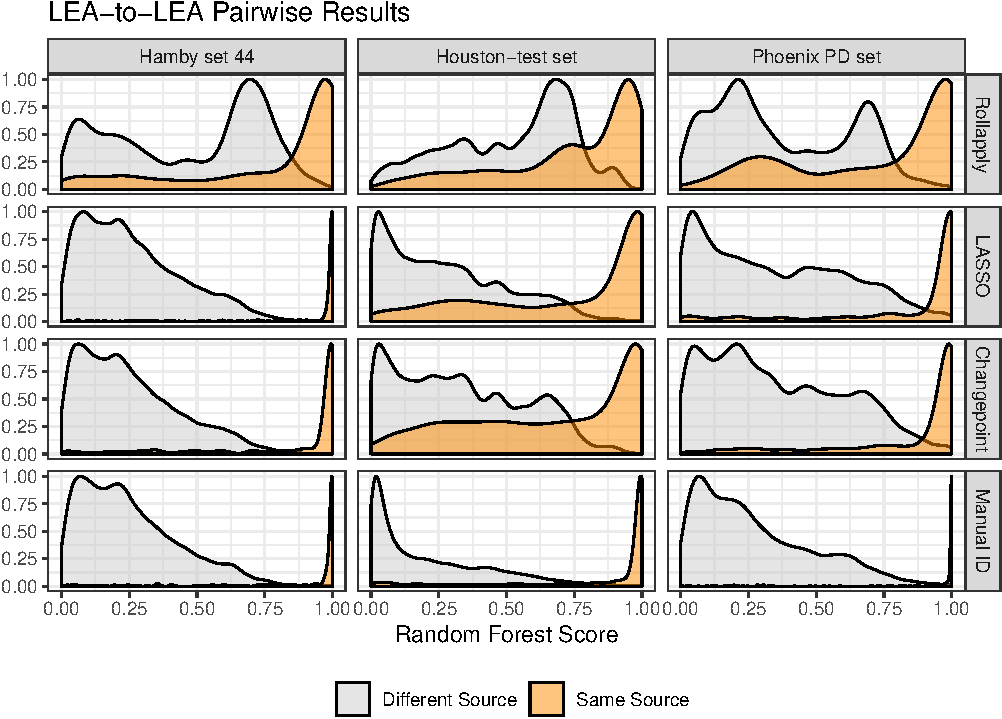
\includegraphics{writeup_files/figure-latex/all-results-1.pdf}
\caption{\label{houston-groove-results}Random forest score distributions
for same source and different source land-to-land comparisons for all
test sets. Logistic LASSO demonstrates improvement over Rollapply, but
is still not as well separated as the Manual ID distributions. Bayesian
changepoint demonstrates similar improvement for Hamby set 44 and
Phoenix PD sets, but does not improve as much as the LASSO method for
the Houston-test set.}
\end{figure}

\section{Conclusions}

Both proposed approaches show significant improvement over the
``rollapply'' method proposed by \cite{Hare1}. However, the logistic
LASSO method shows greater improvement than Bayesian changepoint on the
Houston-test set. While manual identification of shoulder locations is
still the most accurate method, and considered the ``gold standard'',
the reduction in time to get predictions when using LASSO methods is
advantageous and allows for less human involvement in the overall
automated matching process.

The initial appeal of unsupervised methods such as Bayesian changepoint
was the lack of dependence on training data and hence, potential
generalizability advantages. This advantage did not bear out in the test
sets presented here, and it appears the LASSO method trained on Hamby
set 44 generalized effectively to new data.

While improvement is apparent on all three test sets using the LASSO and
Bayesian changepoint methods, there is clear room for additional
precision. Future work on the LASSO method should include re-training
the LASSO model on a wider variety of LEA types rather than just the
Hamby set 44 to avoid over-fitting to a specific type of LEA.

\section{Appendix}

\subsection{MCMC Details}

As a practical note, it turns out that the posterior distribution is
almost always multimodal, and it can happen that the sampler gets stuck
in a suboptimal mode for a large number of iterations. It is also the
case that the suboptimal modes need not even be close to the groove
locations. It has, however, been our experience that the optimal mode
corresponds well to the actual groove locations, which are often
somewhat close to the edges of the data. With this in mind, starting
values and the RWMH proposal variances play a very important role in the
success of the sampling algorithm. Fortunately, it seems to be the case
that by setting the initial changepoint values close to the edges of the
data and making the proposal variance small (around 100 seems to work
well) allows the sampler to wander inwards, and even with a modest
number of iterations (say 5000), typically pass through the largest mode
corresponding to the groove locations. This is not always the case, and
it is possible that increasing the number of iterations produces better
results.

In our implementation of this algorithm, the sampling functions were
originally written with the intention of tuning the proposal variances
to potentially accelerate convergence, and thus several warm-up
iterations are required for this purpose. The concept of warm-up
iterations and tuning proposal variances based on warm-up iterations is
described in Chapter 12.2 of \citet{gelman2013}. This turns out to be a
bad idea in this context for two reasons. The first reason is that the
warm-up iterations allow the sampler to wander past the global modes and
get stuck in suboptimal modes far from the groove locations, from which
the sampler may or may not find its way back to the optimal modes in
just a few thousand iterations. Secondly, if the sampler does wander
past the optimal modes, which are usually on the edges of the data, the
tuned proposal variance can be quite large. The large proposal variance
might not be a huge problem if it weren't for the fact that the width of
the modes are almost always quite small. This means that it can take a
very, very long time for the sampler to move from a suboptimal mode to
the global mode. In order to mitigate this problem, we are currently
setting the number of warmup iterations to be relatively small
(somewhere in 100 to 500 seems to work well). In future, our
implementation of the algorithm will not require any warmup iterations.

Initially, the Metropolis proposal variance for each \(\theta_i\) is
diagonal with diagonal elements all equal to \(1/2\). The proposal
variance for \((c_l, c_r)\) is initially set to be diagonal with
elements equal to \(10^2\). Note that because of the currently necessary
warmup iterations, the variances after warmup for each \(\theta_i\)
becomes
\(\frac{2.4^2}{d}\hat{Var}(\theta_i^{(1:w)}) + \text{diag}(0.1)\), where
\(d\) is the dimension of \(\theta_i\) (which is not constant between
GEAs and LEA), and \(\hat{Var}(\theta_i^{(1:w)})\) is the estimated
variance covariance matrix from the \(w\) warmup iterations. Note that
the approximately optimal proposal variance as described in Chapter 12.2
of \citet{gelman2013} is \(\frac{2.4^2}{d}\hat{Var}(\theta_i^{(1:w)})\).
The addition of a diagonal matrix with entries \(0.1\) is to avoid the
case when most or all warmup iterations have the same value. Similarly,
the proposal variance for \((c_l, c_r)\) after warmup becomes
\(\frac{2.4^2}{2}\hat{Var}((c_l,c_r)^{(1:w)}) + \text{diag}(1)\).

\subsection{Data Preprocessing for MCMC}

Before running the MCMC to do the changepoint detection, we first
perform two data preprocessing steps. The first step is to scale the
residuals from the robust loess procedure by the standard deviation
calculated from the entire set of residuals. The reason for this is
simply to make priors for standard deviation and slope parameters easier
to specify. For example, ensuring that the residuals are scaled to have
standard deviation one means that the standard deviation parameters in
our model should also be close to one. This scaling also ensures that
slopes values are not very large.

The second preprocessing step is a bit more involved. In order to enable
the algorithm to run reasonably fast, we need to take advantage of the
sparse precision matrix structure that is induced by the exponential
covariance function. Indeed, this was the reason for choosing this
covariance function in the first place. Unfortunately, it is challenging
to do this unless the observations are evenly spaced in the domain. In
our case, this would be true if there were no missing values. In order
to remedy this problem, we impute the missing data, but only in the case
that there exist non-missing observations outside of the missing values.
In the case that the missing values exist on the edges of the data, we
simply do not consider those domain values in the model.

We perform the imputation by treating the observations as coming from an
unknown function, and infer the missing values from the known function
values. In order to do this, we model the data with a Gaussian process
and the squared exponential covariance function. That is, we suppose
that

\[
Y(x) \sim \mathcal{GP}(0, K(x,x';\sigma^2, \ell)),
\]

\noindent where now
\(K(x,x';\sigma^2, \ell) = \sigma^2 e^{-(x - x')^2/(2\ell^2)}\) is the
squared exponential covariance function. We emphasize for clarity that
this is a different covariance function than we use in the changepoint
model. The main reason for this is that in imputing values, it seems
desirable to allow dependencies beyond immediately neighboring points to
influence predictions as the function that we are trying to predict
generally has a smooth global structure. For all of our experiments, we
set \(\sigma = 0.8\) and \(\ell = 15\). These values were chosen from
doing maximum likelihood estimation for a representative bullet.

When we impute the missing values, we compute the conditional mean of
the missing values. To be clear, denote the distribution of the observed
and missing data as

\[ 
(Y,Y^*)^\top \sim N\left( \begin{bmatrix} 0 \\ 0 \end{bmatrix}, \begin{bmatrix} \Sigma_{yy} & \Sigma_{yy^*} \\ \Sigma_{y^*y} & \Sigma_{y^*y^*}\end{bmatrix} \right).
\]

\noindent Here, \(Y\) is observed data and \(Y^*\) is the missing data,
and the covariance matrix above is constructed from the squared
exponential covariance function. We then use normal distribution theory
to calculate the imputed values

\[ E(Y^*|Y = y) = \Sigma_{y^*y} \Sigma_{yy}^{-1}y \].

\bibliographystyle{jfs-authoryear}
\bibliography{bibliography}

\end{document}